\documentclass{beamer}
\usepackage[latin1]{inputenc}
\usepackage{times}
\usepackage{tikz}
\usetheme{Luebeck}
%\usecolortheme{albatross}
\usepackage{amsmath,amsfonts,amsthm,amssymb}
\usepackage{setspace}
\usepackage{Tabbing}
\usepackage{fancyhdr}
\usepackage{lastpage}
\usepackage{extramarks}
\usepackage{chngpage}
\usepackage{soul,color}
\usepackage{graphicx,float,wrapfig}
\usepackage{listings}
\usepackage{float}
\usepackage{subfigure}
\usepackage{enumitem}
\usepackage{algpseudocode}

\definecolor{darkorange}{RGB}{240, 120, 0}

\setbeamercolor{background canvas}{bg=white}
\setbeamercolor{frametitle}{fg=white, bg=darkorange}
\setbeamercolor{normal text}{bg=black,fg=black}
\setbeamercolor{structure}{bg=black, fg=darkorange}

\title{Lecture 4: Planes, Interior Point Testing, Duality}
\date{1/26/2016}
\institute{Chris Tralie, Duke University}
\author{COMPSCI/MATH 290-04}
\begin{document}

\frame{\titlepage}


%Intro: Preview of loop ditty: 
%How did we get that?  What can we do with it?  Where are we in practice?
%First goal: perceptually-motivated 

\begin{frame}{Table of Contents}

\begin{itemize}[label=$\blacktriangleright$]
	\item Normals and Planes
\end{itemize}
\begin{itemize}[label=$\vartriangleright$]
    \item Interior Point Testing
    \item Duality
%    \item Voronoi Diagrams
\end{itemize}

\end{frame}

\begin{frame}{Announcements}

\begin{itemize}[label=$\blacktriangleright$]
    \item Everyone got Mini 1 Part 1 in on time!
    \item Part 2 Due Friday 11:55 PM
    \item Drop/Add Tomorrow!
    \item SIGGRAPH Student Volunteers application 
    \small
    \url{http://s2016.siggraph.org/student-volunteers}
\end{itemize}

\end{frame}

\begin{frame}{Normals}
\begin{itemize}[label=$\vartriangleright$]
    \item Vector in direction perpendicular to object in question
\end{itemize}

\begin{figure}[t]
	\centering
	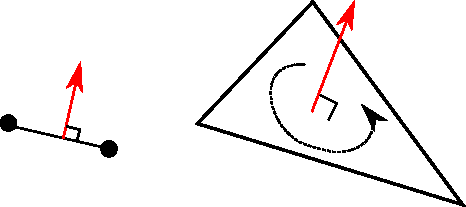
\includegraphics[width=1\textwidth]{NormalExamples.pdf}
\end{figure}

\end{frame}

\begin{frame}{Perpendicular To A 2D Vector}
\begin{itemize}[label=$\vartriangleright$]
    \item Negate y and swap: $(a, b) \rightarrow (-b, a)$
\end{itemize}

\begin{figure}[t]
	\centering
	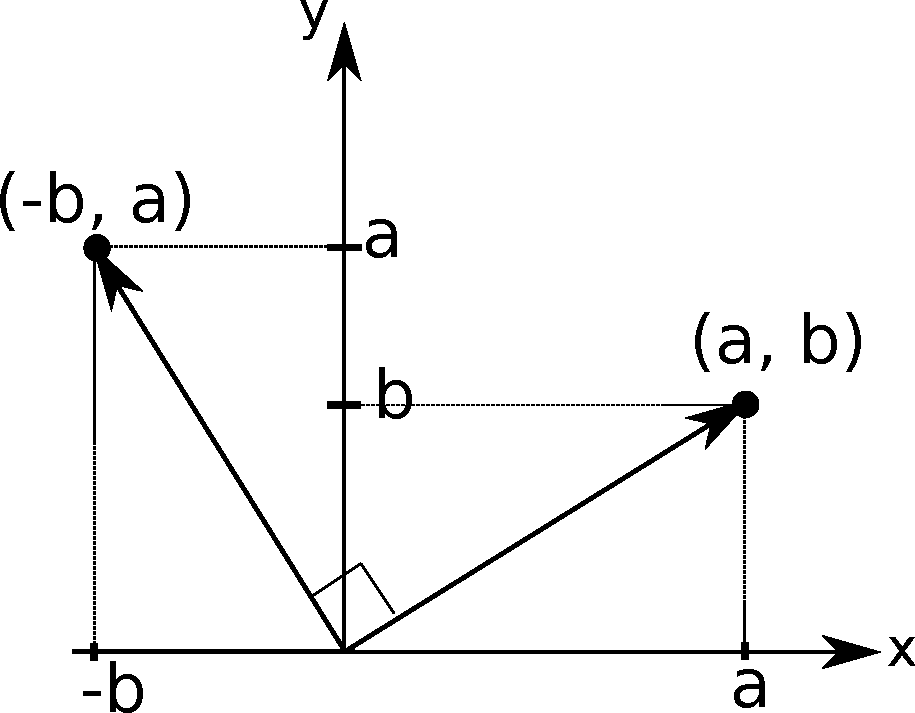
\includegraphics[width=0.7\textwidth]{VectorPerp.pdf}
\end{figure}

\end{frame}



\begin{frame}{Normal Form of A Line}

Given point $\vec{p}$ and normal $\vec{n}$, a point $\vec{q}$ is on line if
\[ (\vec{q} - \vec{p}) \cdot \vec{n} = 0 \]

\begin{figure}[t]
	\centering
	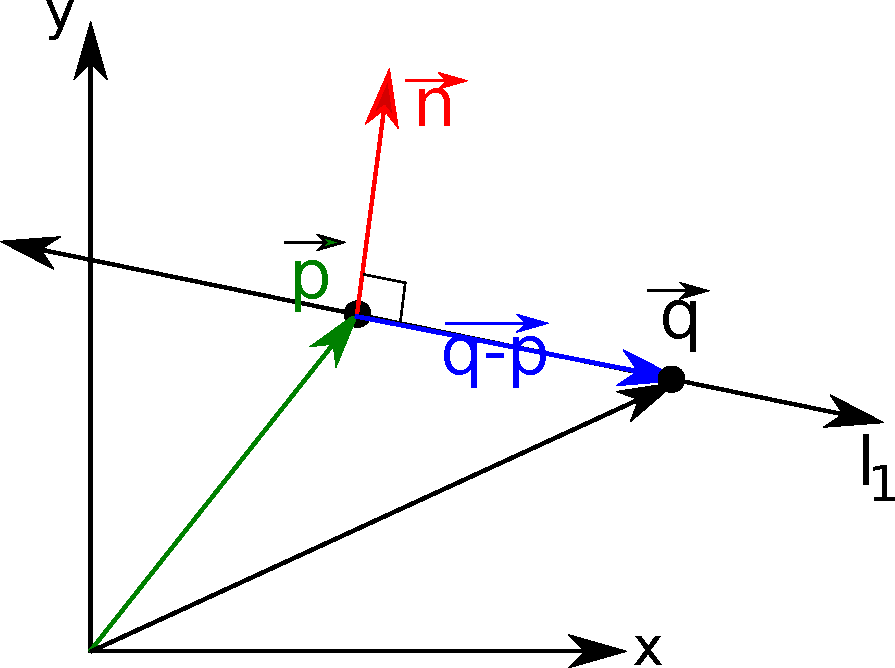
\includegraphics[width=0.6\textwidth]{LineNormalForm.pdf}
\end{figure}

\end{frame}

\begin{frame}{Normal Form of A Line}
\[ (\vec{q} - \vec{p}) \cdot \vec{n} = 0 \]

Assume $||\vec{n}|| = 1$ (unit normal)

\[ \vec{q} \cdot \vec{n} = \vec{p} \cdot \vec{n} = d(l_1, \text{origin}) \]



\begin{figure}[t]
	\centering
	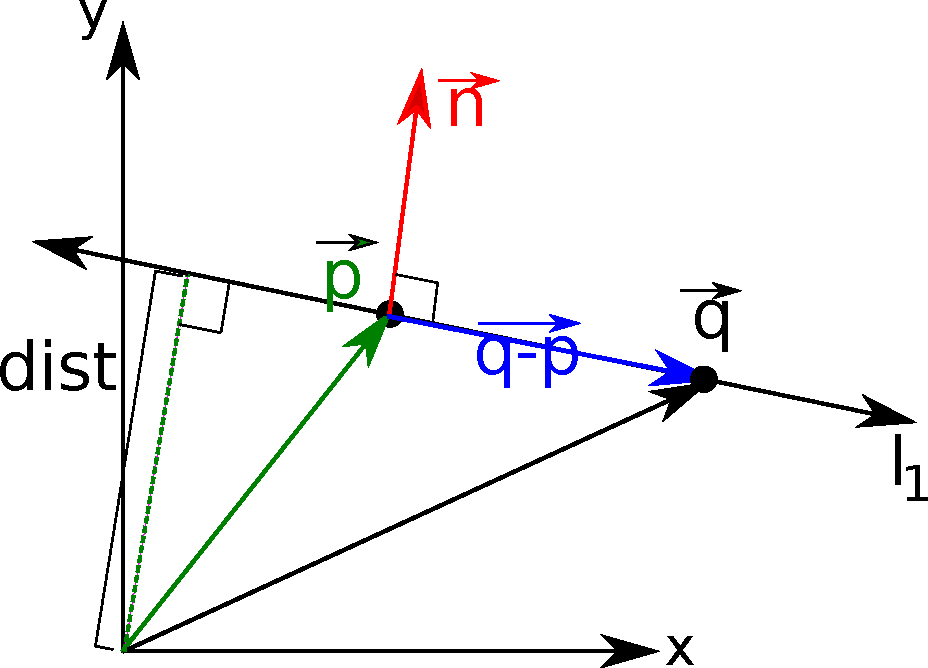
\includegraphics[width=0.6\textwidth]{LineNormalFormDist.pdf}
\end{figure}

\end{frame}


\begin{frame}{Normal Form of A Line}
\[ (\vec{q} - \vec{p}) \cdot \vec{n} = 0 \]

Let $q = (x, y)$.  Expanding and rewriting as implicit linear equation

\[ n_x x + n_y y - d(l_1, \text{origin}) = 0 \]



\begin{figure}[t]
	\centering
	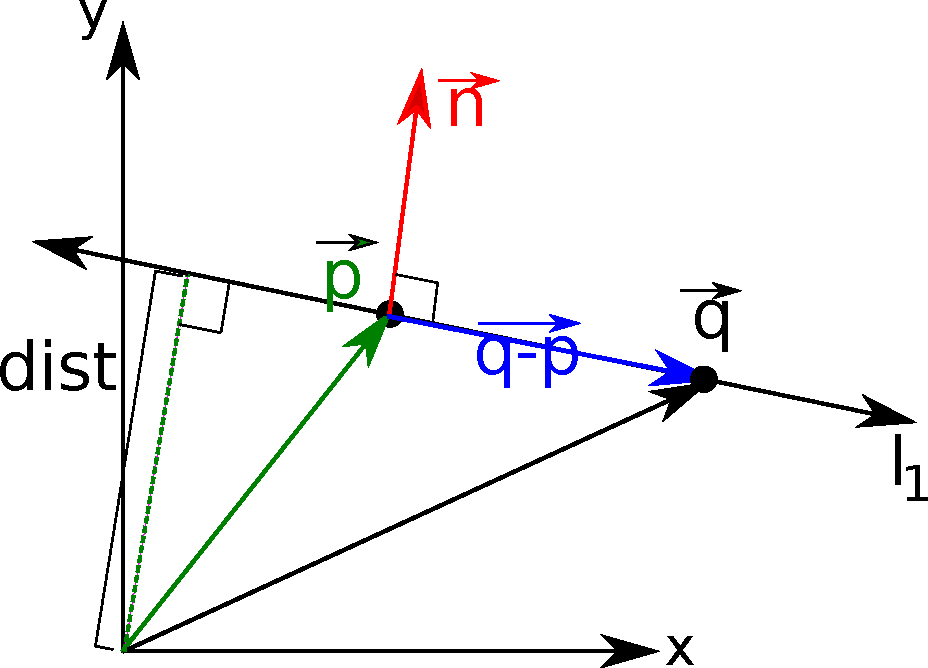
\includegraphics[width=0.6\textwidth]{LineNormalFormDist.pdf}
\end{figure}

\end{frame}

\begin{frame}{Line: Degrees of Freedom}

\[ n_x x + n_y y - d(l_1, \text{origin}) = 0 \]

\[ Ax + By + C = 0 \]

Implicit form

\begin{itemize}[label=$\vartriangleright$]

\item How many {\em degrees of freedom} are there in a line?

\end{itemize}

\end{frame}


\begin{frame}{Normal Form of a Line}


\begin{itemize}[label=$\vartriangleright$]

\item What's the line normal of the line $y = mx + b$?

\end{itemize}

\end{frame}


\begin{frame}{2D Planes}

Given point $\vec{p}$ and normal $\vec{n}$, a point $\vec{q}$ is on plane if
\[ (\vec{q} - \vec{p}) \cdot \vec{n} = 0  \implies \vec{q} \cdot \vec{n} = \vec{p} \cdot \vec{n} = 0\]
(now 3D vectors)

\begin{figure}[t]
	\centering
	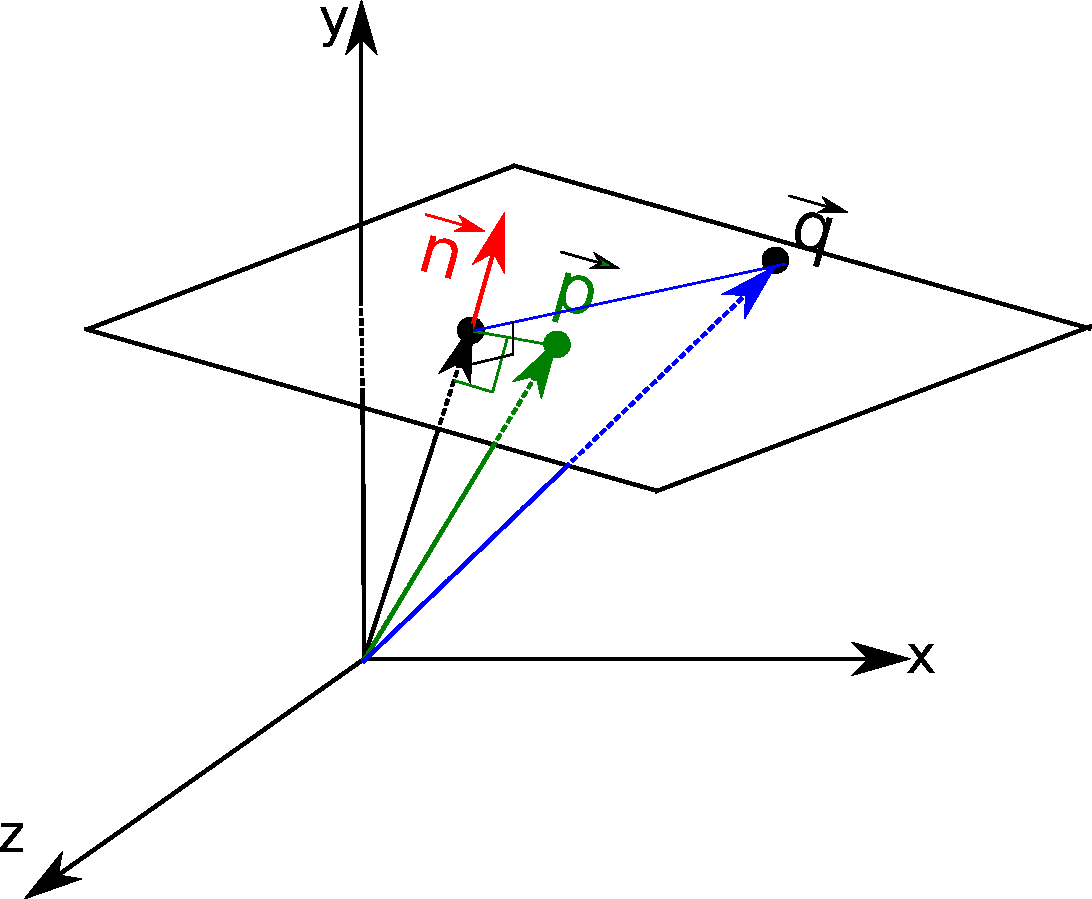
\includegraphics[width=0.6\textwidth]{PlaneNormalForm.pdf}
\end{figure}

\end{frame}


\begin{frame}{2D Planes}

\[ n_x x + n_y y + n_z z - d(p, \text{origin}) = 0 \]

\begin{figure}[t]
	\centering
	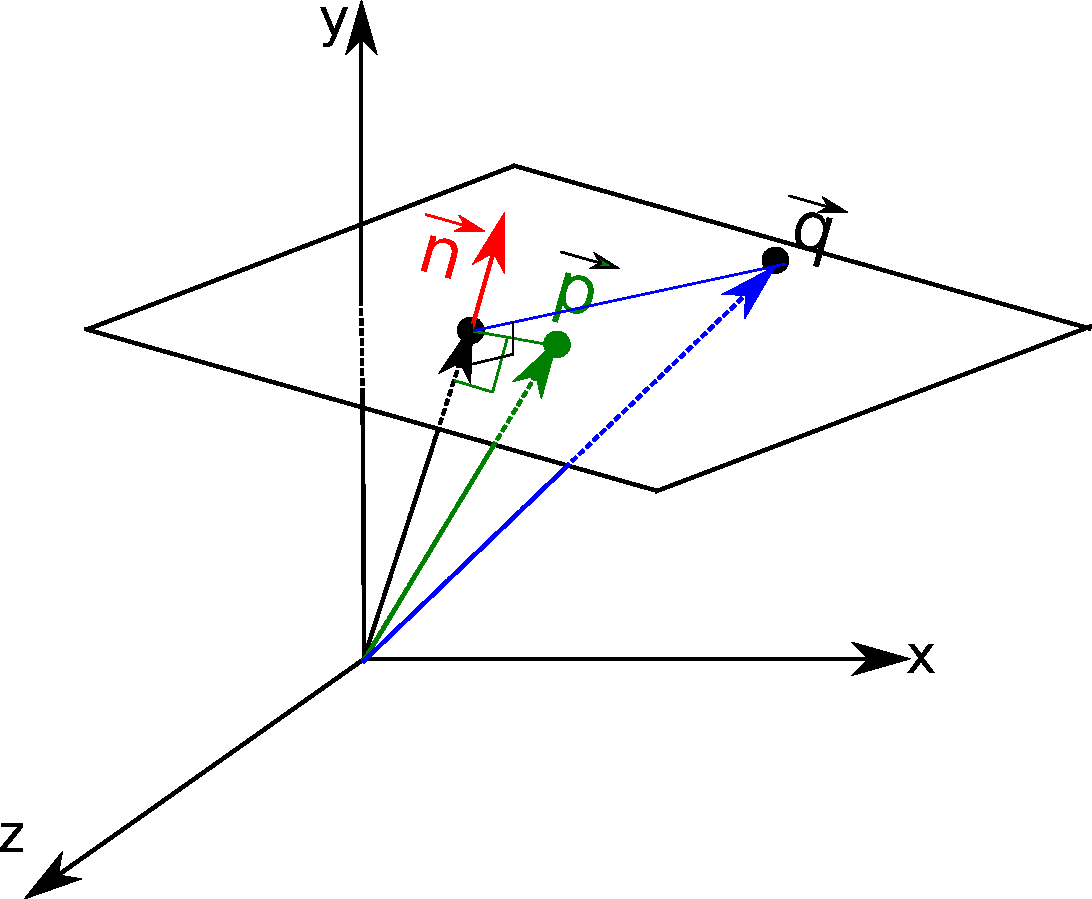
\includegraphics[width=0.6\textwidth]{PlaneNormalForm.pdf}
\end{figure}

\end{frame}


\begin{frame}{2D Planes}

\[Ax + By + Cz + D = 0 \]

\begin{figure}[t]
	\centering
	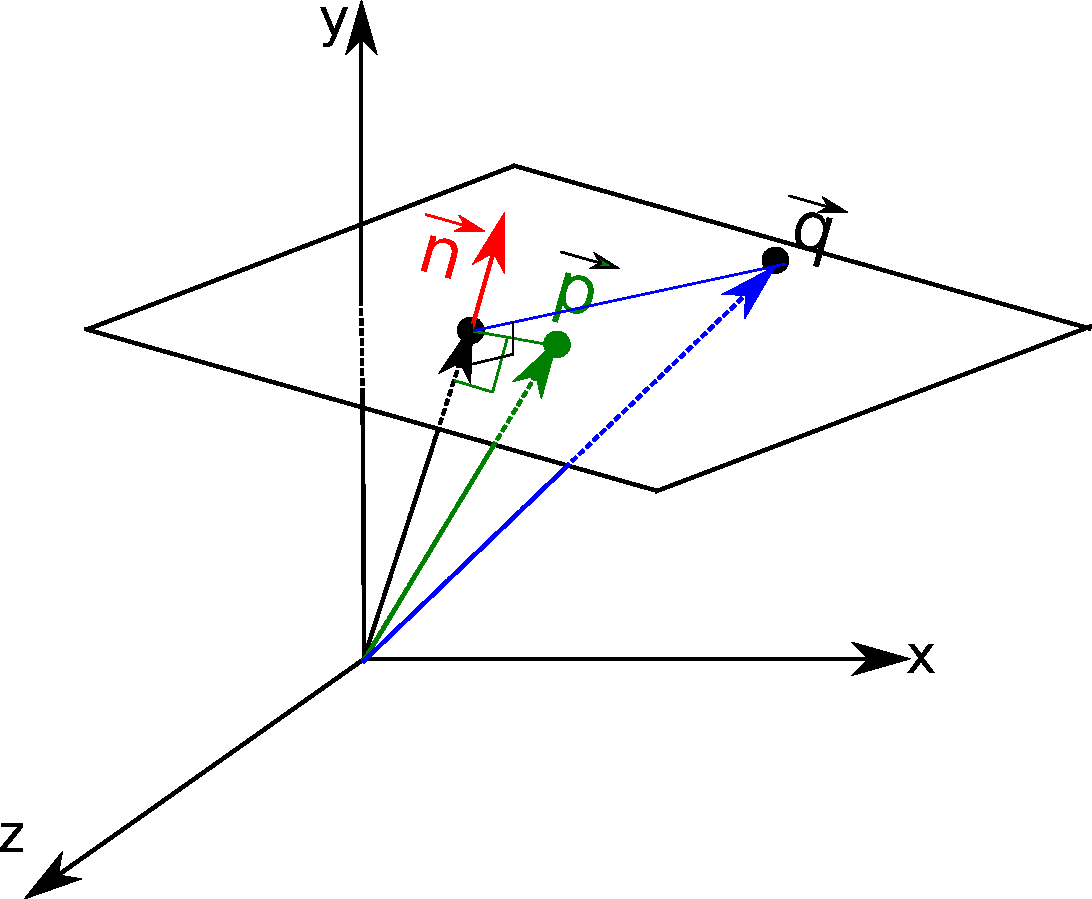
\includegraphics[width=0.6\textwidth]{PlaneNormalForm.pdf}
\end{figure}


\end{frame}


\begin{frame}{Ray Intersect Plane}

\begin{figure}[t]
	\centering
	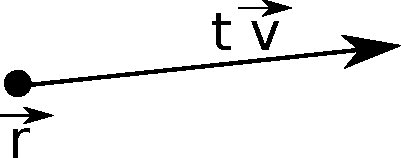
\includegraphics[width=0.4\textwidth]{ray.pdf}
\end{figure}

Plane: $ (\vec{q} - \vec{p}) \cdot \vec{n} = 0 $

Ray: $ \vec{r} + t \vec{v}, t \geq 0 $

\[ t = \frac{ - \vec{r} \cdot \vec{n}}{\vec{v} \cdot \vec{n}}\]

\end{frame}



%%%%%%%%%%% Section 2: Interior Point Testing

\begin{frame}{Table of Contents}

\begin{itemize}[label=$\vartriangleright$]
	\item Normals and Planes
\end{itemize}
\begin{itemize}[label=$\blacktriangleright$]
    \item Interior Point Testing
\end{itemize}
\begin{itemize}[label=$\vartriangleright$]
    \item Duality
%    \item Voronoi Diagrams
\end{itemize}

\end{frame}

\begin{frame}{Convex Polygons}

\begin{figure}[t]
	\centering
	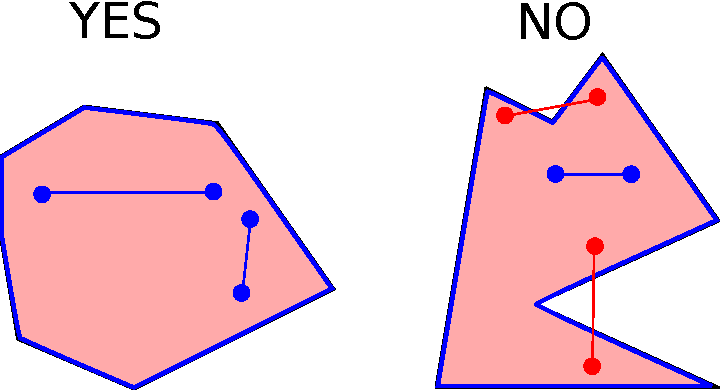
\includegraphics[width=1\textwidth]{ConvexNonconvex.pdf}
\end{figure}

Definition extends to 3D polytopes (and any geometric set)

\end{frame}


\begin{frame}{Convex Or Not?}

\begin{figure}[t]
	\centering
	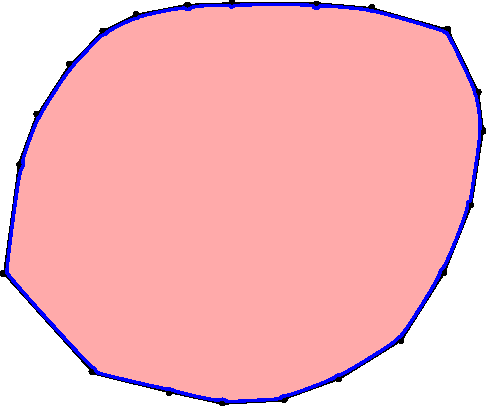
\includegraphics[width=0.7\textwidth]{ConvexNonconvex1.pdf}
\end{figure}

\end{frame}


\begin{frame}{Convex Or Not?}

\begin{figure}[t]
	\centering
	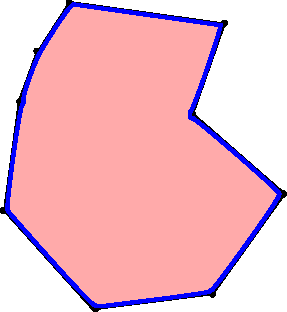
\includegraphics[width=0.5\textwidth]{ConvexNonconvex2.pdf}
\end{figure}

\end{frame}

\begin{frame}{Convex Or Not?}

\begin{figure}[t]
	\centering
	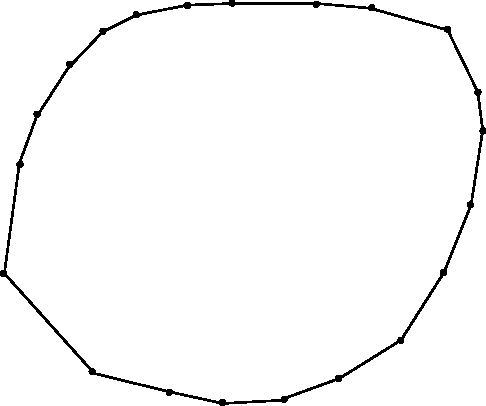
\includegraphics[width=0.7\textwidth]{ConvexNonconvex3.pdf}
\end{figure}

\end{frame}

%Triangles first (area method works for any convex polygon)

\begin{frame}{Point Inside Convex Polygon: Halfplane Method}

\begin{figure}[t]
	\centering
	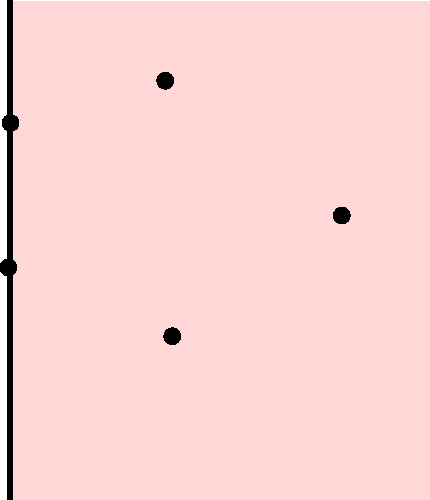
\includegraphics[width=0.75\textwidth]{Halfplane1.pdf}
\end{figure}

\end{frame}

\begin{frame}{Point Inside Convex Polygon: Halfplane Method}

\begin{figure}[t]
	\centering
	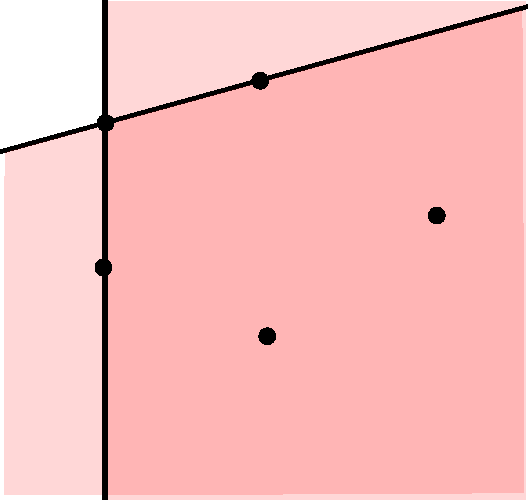
\includegraphics[width=\textwidth]{Halfplane2.pdf}
\end{figure}

\end{frame}

\begin{frame}{Point Inside Convex Polygon: Halfplane Method}

\begin{figure}[t]
	\centering
	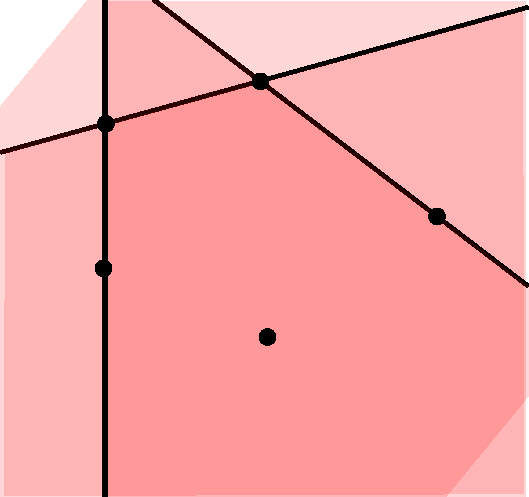
\includegraphics[width=\textwidth]{Halfplane3.pdf}
\end{figure}

\end{frame}

\begin{frame}{Point Inside Convex Polygon: Halfplane Method}

\begin{figure}[t]
	\centering
	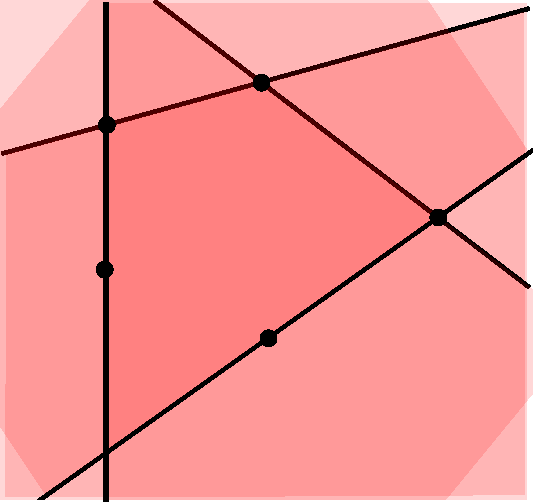
\includegraphics[width=\textwidth]{Halfplane4.pdf}
\end{figure}

\end{frame}

\begin{frame}{Point Inside Convex Polygon: Halfplane Method}

\begin{figure}[t]
	\centering
	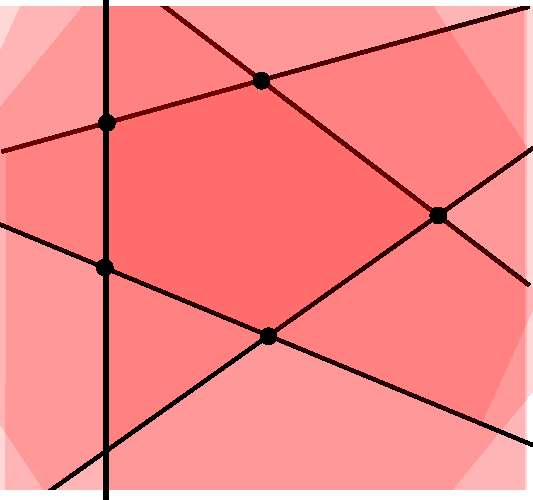
\includegraphics[width=\textwidth]{Halfplane5.pdf}
\end{figure}

\end{frame}


\begin{frame}{Point Inside Convex Polygon: Hull Method}

Convex Hull (Segue) 

\begin{figure}[t]
	\centering
	
\includegraphics[width=0.7\textwidth]{ConvexHullExample.pdf}
\end{figure}


\end{frame}


\begin{frame}{Point Inside Convex Polygon: Hull Method}

Convex Hull (Segue) 

\begin{figure}[t]
	\centering
	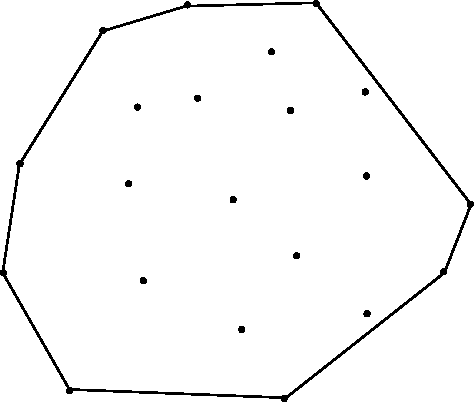
\includegraphics[width=0.7\textwidth]{ConvexHullExample2.pdf}
\end{figure}


\end{frame}

\begin{frame}{Point Inside Convex Polygon: Hull Method}

Convex Hull Test

\begin{figure}[t]
	\centering
	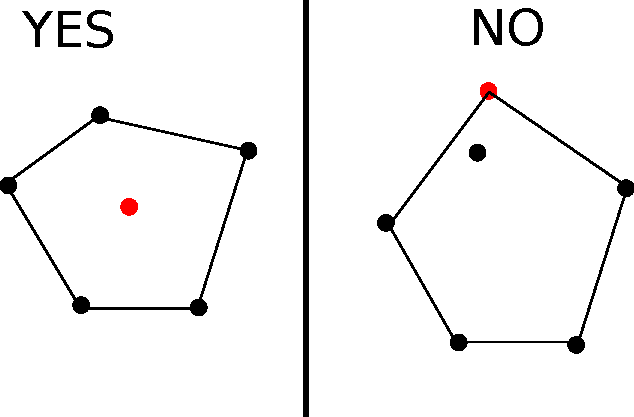
\includegraphics[width=\textwidth]{ConvexHullTest.pdf}
\end{figure}

\end{frame}



\begin{frame}{Point Inside Convex Polygon: Area Method}


\[ \text{Area}(\triangle abc) = \text{Area}(\triangle abd) + \text{Area}(\triangle bcd) + \text{Area}(\triangle cad)\]

\begin{figure}[t]
	\centering
	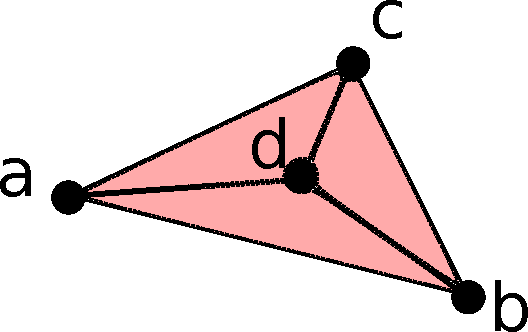
\includegraphics[width=0.8\textwidth]{PointInsideArea.pdf}
\end{figure}


\end{frame}


\begin{frame}{Point Inside Convex Polygon: Area Method}


\[ \text{Area}(\triangle abc) < \text{Area}(\triangle abd) + \text{Area}(\triangle bcd) + \text{Area}(\triangle acd)\]

\begin{figure}[t]
	\centering
	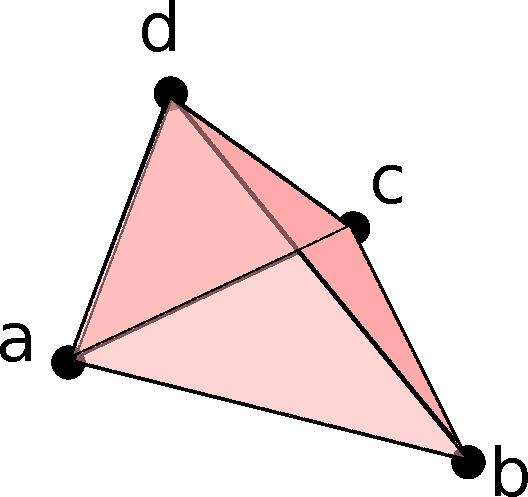
\includegraphics[width=0.5\textwidth]{PointOutsideArea1.pdf}
\end{figure}


\end{frame}


\begin{frame}{Point Inside Convex Polygon: Area Method}




\end{frame}

\begin{frame}{3D Ray Convex Polygon Intersection}

\begin{figure}[t]
	\centering
	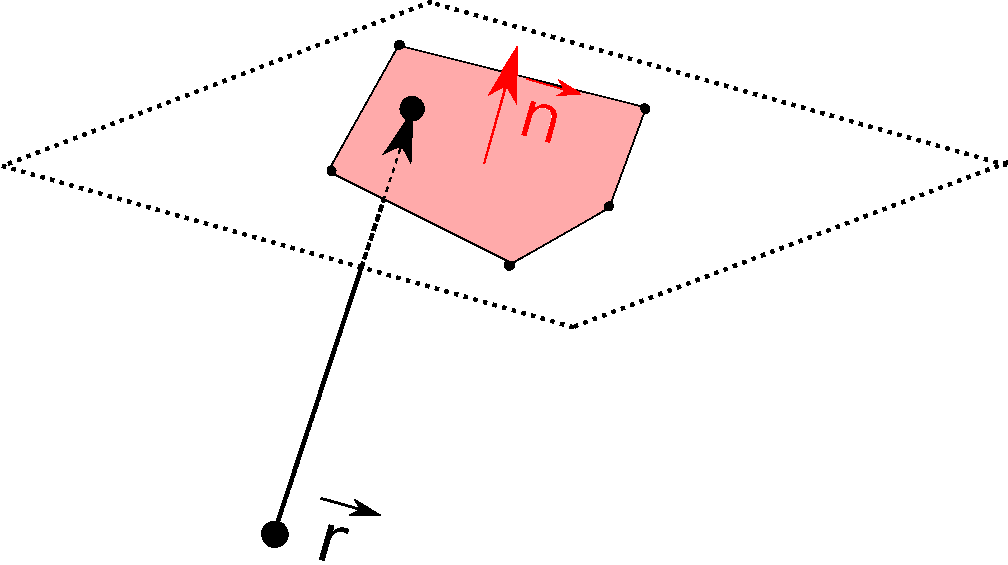
\includegraphics[width=\textwidth]{PolygonRayIntersect.pdf}
\end{figure}


\end{frame}



\begin{frame}{Logarithmic Convex Polygon Test}

\begin{figure}[t]
	\centering
	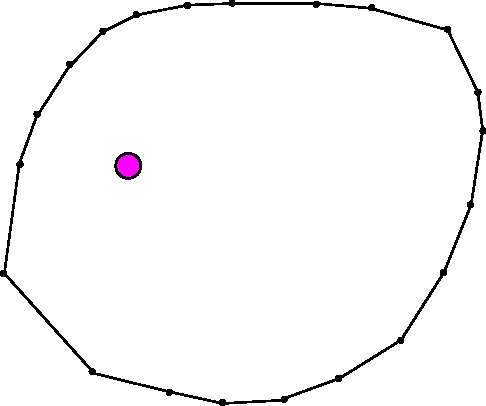
\includegraphics[width=0.6\textwidth]{ConvexPolygon.pdf}
\end{figure}

\end{frame}


\begin{frame}{Logarithmic Convex Polygon Test}

Segue: Binary Search

\end{frame}

\begin{frame}{Logarithmic Convex Polygon Test}

\begin{figure}[t]
	\centering
	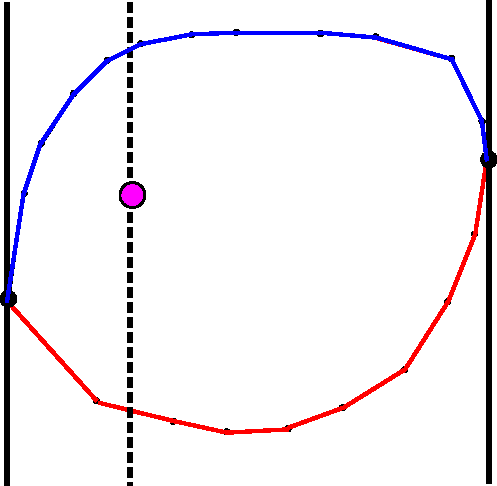
\includegraphics[width=0.6\textwidth]{ConvexPolygonCastLines.pdf}
\end{figure}

\end{frame}


\begin{frame}{Logarithmic Convex Polygon Test}

\begin{figure}[t]
	\centering
	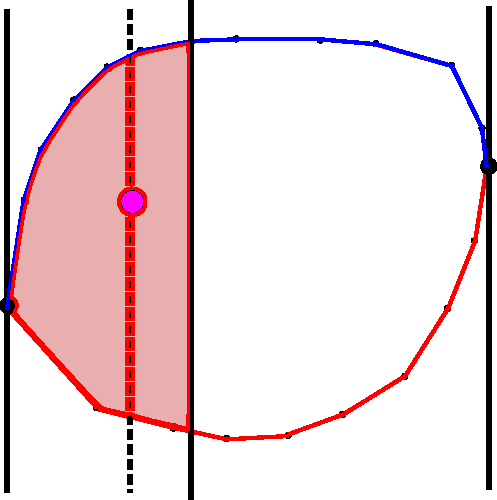
\includegraphics[width=0.6\textwidth]{ConvexPolygonCastLines1.pdf}
\end{figure}

\end{frame}



\begin{frame}{Logarithmic Convex Polygon Test}

\begin{figure}[t]
	\centering
	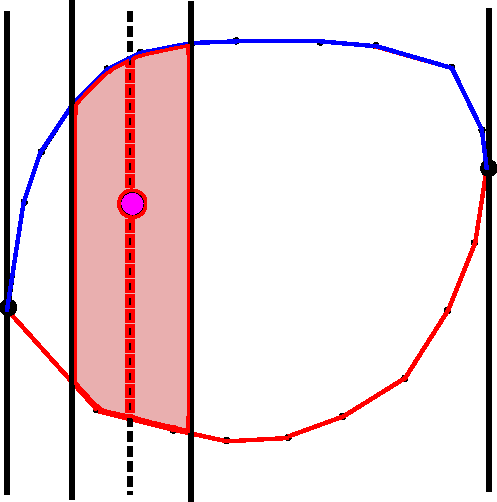
\includegraphics[width=0.6\textwidth]{ConvexPolygonCastLines2.pdf}
\end{figure}

\end{frame}


\begin{frame}{Logarithmic Convex Polygon Test}

\begin{figure}[t]
	\centering
	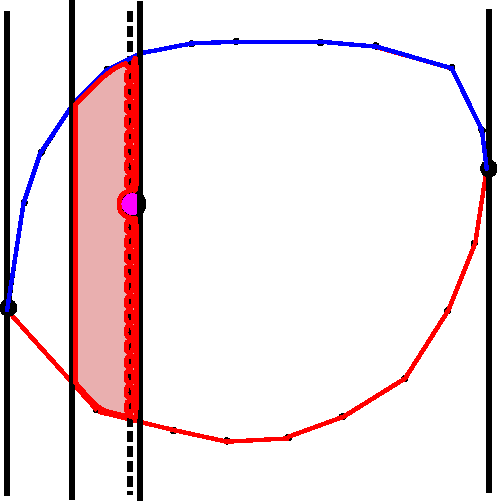
\includegraphics[width=0.6\textwidth]{ConvexPolygonCastLines3.pdf}
\end{figure}

\end{frame}

\begin{frame}{Logarithmic Convex Polygon Test}

\begin{figure}[t]
	\centering
	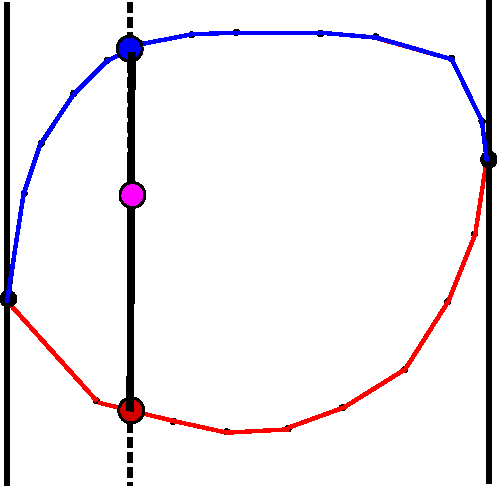
\includegraphics[width=0.6\textwidth]{ConvexPolygonCastLinesIntersect.pdf}
\end{figure}

\end{frame}



\begin{frame}{Nonconvex Polygons}

Inside or outside??

\begin{figure}[t]
	\centering
	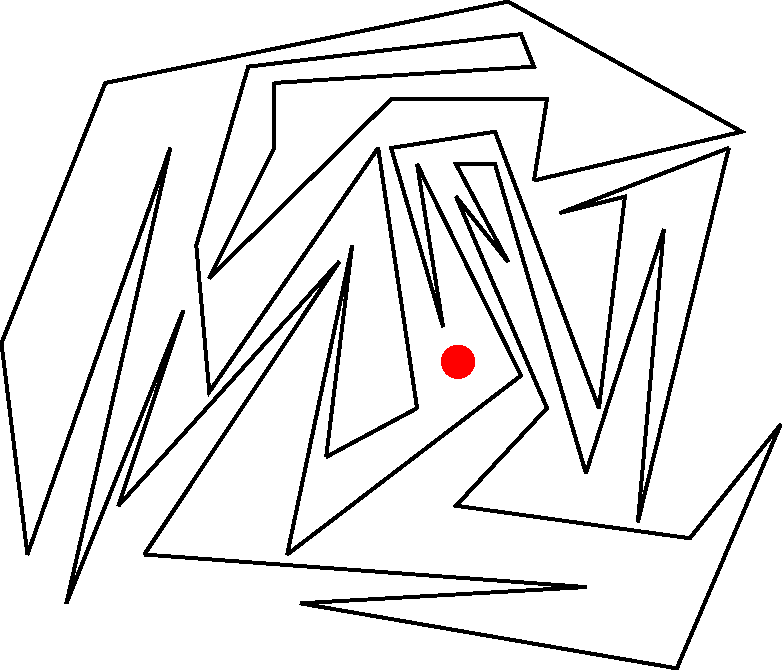
\includegraphics[width=0.8\textwidth]{SimplePolygon1.pdf}
\end{figure}

\end{frame}

\begin{frame}{Nonconvex Polygons}

\begin{figure}[t]
	\centering
	
\includegraphics[width=0.8\textwidth]{SimplePolygon1Filled.pdf}
\end{figure}

\end{frame}


\begin{frame}{Nonconvex Polygons: Ray Casting}

\begin{figure}[t]
	\centering
	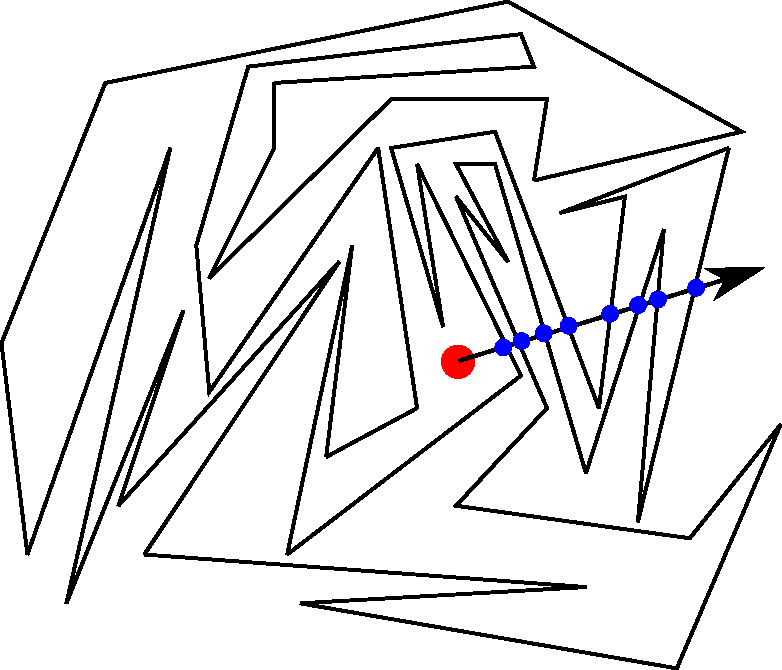
\includegraphics[width=0.8\textwidth]{SimplePolygon1Ray.pdf}
\end{figure}

\end{frame}


%Section 3: Duality

\begin{frame}{Table of Contents}

\begin{itemize}[label=$\vartriangleright$]
	\item Normals and Planes
    \item Interior Point Testing
\end{itemize}
\begin{itemize}[label=$\blacktriangleright$]
    \item Duality
%    \item Voronoi Diagrams
\end{itemize}

\end{frame}


\begin{frame}{Points To Lines}

\begin{figure}[t]
	\centering
	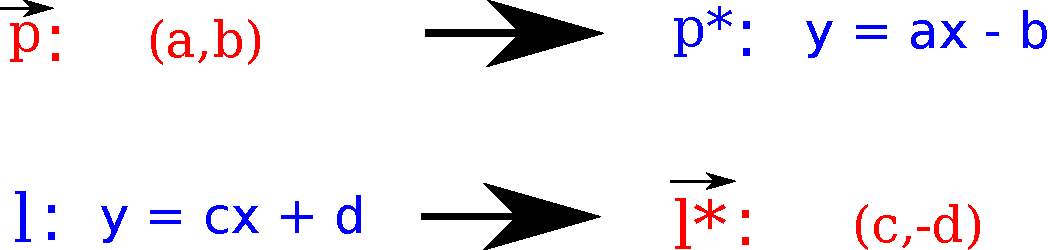
\includegraphics[width=\textwidth]{dualityEquations.pdf}
\end{figure}

\end{frame}



\begin{frame}{Points To Lines}


\[ \vec{p} > l  \iff \vec{l^*} > p^* \]


where $``>"$ means ``above"

TODO: Verify this using vectors!

\begin{figure}[t]
	\centering
	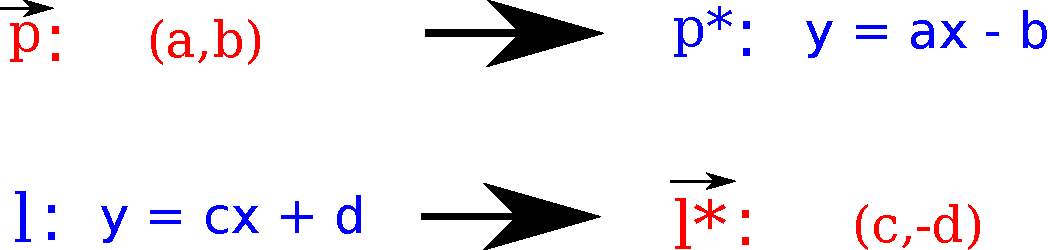
\includegraphics[width=\textwidth]{dualityEquations.pdf}
\end{figure}



\end{frame}

\begin{frame}{Point Inside Convex Polygon: Halfplane Method}

What dual problem did we solve??

\begin{figure}[t]
	\centering
	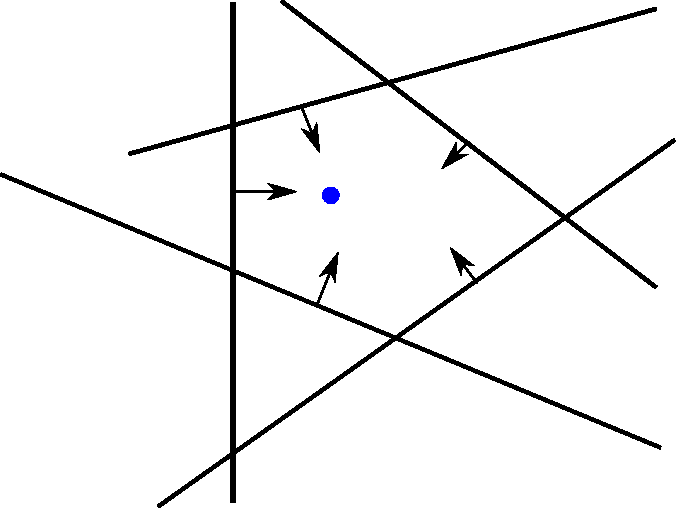
\includegraphics[width=\textwidth]{HalfplanePrimal.pdf}
\end{figure}

\end{frame}


\begin{frame}{Point Inside Convex Polygon: Halfplane Method}

What dual problem did we solve??

\begin{figure}[t]
	\centering
	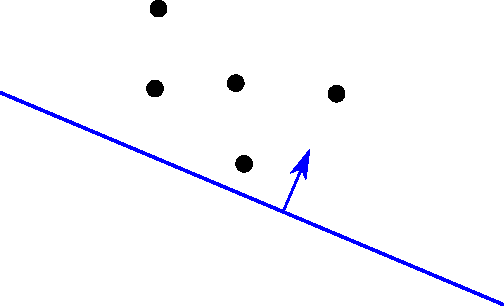
\includegraphics[width=\textwidth]{HalfplaneDual.pdf}
\end{figure}

\end{frame}


%\begin{frame}{Simple Polygons}

%\begin{figure}[t]
%	\centering
%	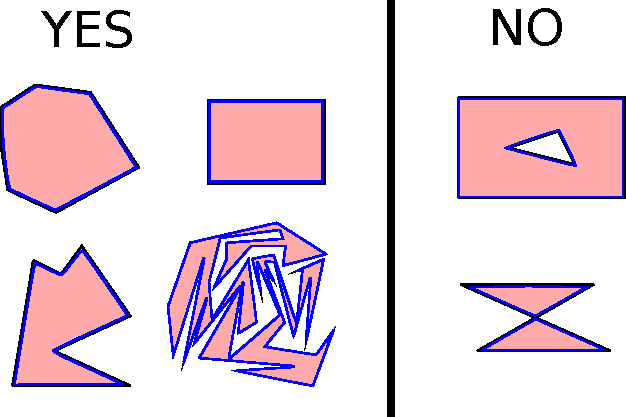
\includegraphics[width=1\textwidth]{SimpleVsNot.pdf}
%\end{figure}

%Definition extends to 3D polytopes

%\end{frame}




\end{document}

